\documentclass[a4paper,12pt]{article} % тип документа

% Поля страниц
\usepackage[left=2.5cm,right=2.5cm, top=2cm,bottom=2cm,bindingoffset=0cm]{geometry}
    
%Пакет дял таблиц   
\usepackage{multirow} 
    
%Отступ после заголовка    
\usepackage{indentfirst}


% Рисунки
\usepackage{subcaption,floatrow,graphicx,calc}
\usepackage{wrapfig}

% Создаёем новый разделитель
\DeclareFloatSeparators{mysep}{\hspace{1cm}}

% Ссылки?
\usepackage{hyperref}
\usepackage[rgb]{xcolor}
\hypersetup{				% Гиперссылки
    colorlinks=true,       	% false: ссылки в рамках
	urlcolor=blue          % на URL
}


%  Русский язык
\usepackage[T2A]{fontenc}			% кодировка
\usepackage[utf8]{inputenc}			% кодировка исходного текста
\usepackage[english,russian]{babel}	% локализация и переносы


% Математика
\usepackage{amsmath,amsfonts,amssymb,amsthm,mathtools, mathrsfs, wasysym}


\begin{document}
\begin{center}
	\footnotesize{ФЕДЕРАЛЬНОЕ ГОСУДАРСТВЕННОЕ АВТОНОМНОЕ ОБРАЗОВАТЕЛЬНОЕ 			УЧРЕЖДЕНИЕ ВЫСШЕГО ОБРАЗОВАНИЯ}\\
	\footnotesize{МОСКОВСКИЙ ФИЗИКО-ТЕХНИЧЕСКИЙ ИНСТИТУТ\\(НАЦИОНАЛЬНЫЙ 			ИССЛЕДОВАТЕЛЬСКИЙ УНИВЕРСИТЕТ)}\\
	\footnotesize{ФАКУЛЬТЕТ ОБЩЕЙ И ПРИКЛАДНОЙ ФИЗИКИ\\}
	\hfill \break
	\hfill\break
	\hfill\break
	\hfill \break
	\hfill \break
	\hfill \break
	\hfill \break
	\hfill \break
	\hfill \break
	\hfill \break
	\hfill \break
	\hfill \break
	\hfill \break
	\hfill \break
	\large{Лабораторная работа № 6.11.3 \\\textbf{Измерение контактной разности потенциалов в полупроводниках}}\\
	\hfill \break
	\hfill \break
	\hfill \break
	\begin{flushright}
		Серебренников Даниил\\
		Группа Б02-826м
	\end{flushright}
	\hfill \break
	\hfill \break
	\hfill \break
	\hfill \break
	\hfill \break
	\hfill \break
	\hfill \break
	\hfill \break
	\hfill \break
	\hfill \break
	\hfill \break
\end{center}
\begin{center}
	Долгопрудный, 2021 г.
\end{center}
\thispagestyle{empty}
\newpage
	\textbf{Цель работы:} определить контактную разность потенциалов (p-n)-перехода в полупроводниковом диоде по результатам измерений температурной зависимости его сопротовиления.

\section{Основные формулы}
	Контактная разность потенциалов полупроводника при комнатных температурах:
	\begin{equation*}
		\label{eq:formula}
		\tag{$\star$}
		\Delta V = \frac{k}{e} \frac{\Delta (\ln R)}{\Delta(1/T)},
	\end{equation*}
	где $k$ -- постоянная больцмана, $e$ -- элементарный заряд, $R$ -- сопротивление полупроводника, $T$ -- его температура.
\section{Экспериментальная установка}
	\thisfloatsetup{floatrowsep=mysep}	
	\begin{figure}[h!]
		\begin{floatrow}
			\ffigbox[\FBwidth]{\caption{Схема экспериментальной установки.}\label{fig:ust}}
				{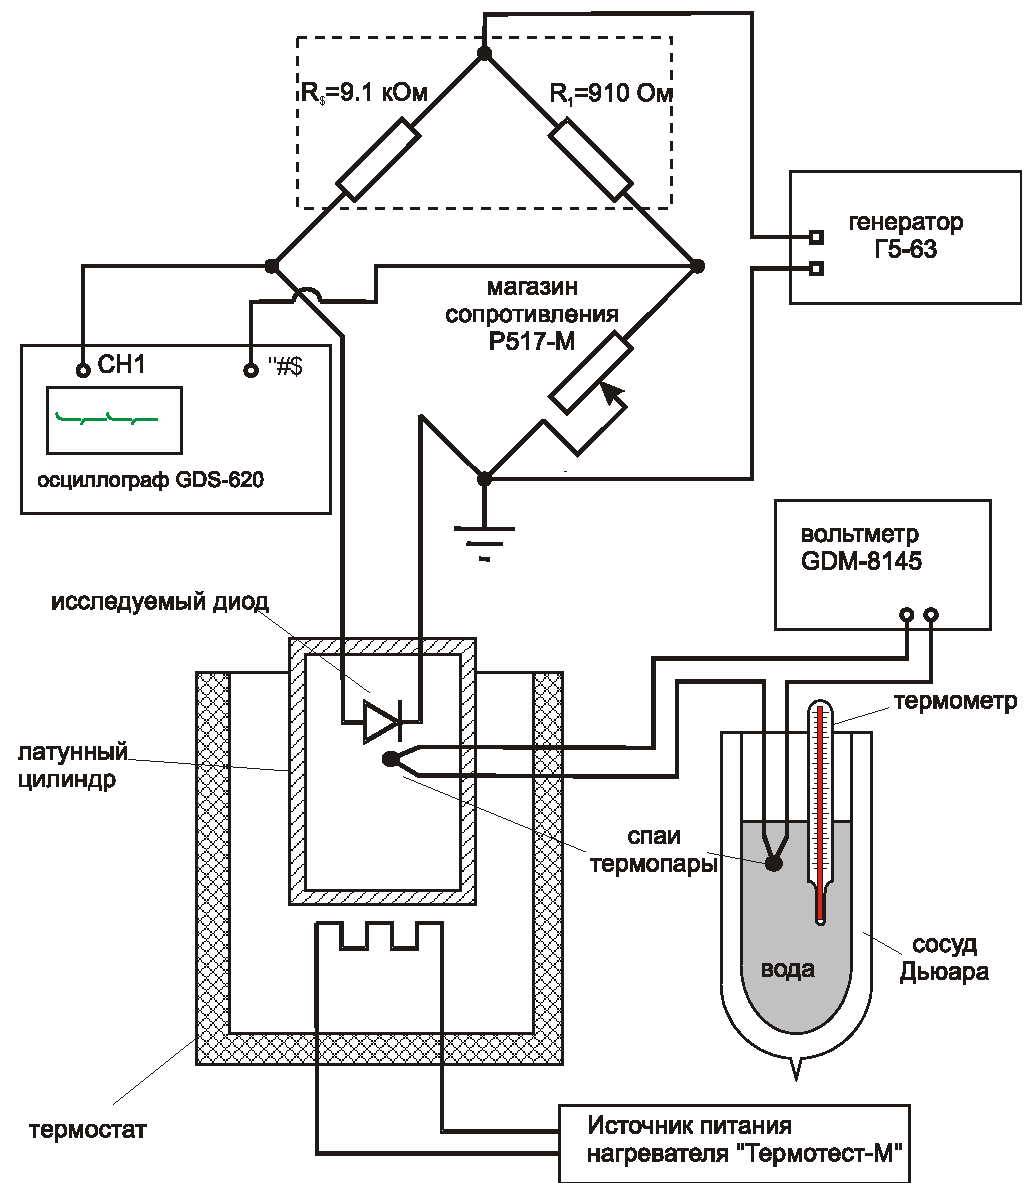
\includegraphics[scale=0.7]{ustanovka.pdf}}    
			\end{floatrow}
		\end{figure}
	
	
	
	\newpage
	\section{Экспериментальные данные}
		\begin{enumerate}
			\item
				Коэффициент термопары:
				$\lambda$ = 41мкВ/$^\circ$;
			\item
				Температура термометра: $t_1 = (24,0 \pm 0,5)^\circ$C;
			\item
				Температура воздуха: $t_2 = (26,0 \pm 0,5)^\circ$C;
			\item
				Погрешность вольтметра $\sigma_V^{(1)} = 10$ мкВ;
			\item
				Сдвиг нуля вольтметра $\sigma_V^{(2)} = 10$ мкВ.
		\end{enumerate}
		
		\floatsetup[table]{capposition=top}	
		\begin{table}[H]
			\caption{Результаты измерений.}
			\label{table:exp1}
			\begin{tabular}{|c|c|c|c|c|c|c|}
				\hline
				$R_M$, Ом & $R_g$, Ом & $V$, мкВ & $t$, $^\circ$C & $T$, К & $1/T$, К$^{-1}$ & $\ln R_g$ \\ \hline
				279,03    & 2790,3    & 80       & 26,0           & 299,0  & 0,003345        & 7,93      \\ \hline
				125,05    & 1250,5    & 440      & 34,7           & 307,7  & 0,003250        & 7,13      \\ \hline
				90,04     & 900,4     & 630      & 39,4           & 312,4  & 0,003201        & 6,80      \\ \hline
				60,57     & 605,7     & 870      & 45,2           & 318,2  & 0,003142        & 6,41      \\ \hline
				50,38     & 503,8     & 1020     & 48,9           & 321,9  & 0,003107        & 6,22      \\ \hline
				41,63     & 416,3     & 1230     & 54,0           & 327,0  & 0,003058        & 6,03      \\ \hline
				22,94     & 229,4     & 1640     & 64,0           & 337,0  & 0,002967        & 5,44      \\ \hline
				18,93     & 189,3     & 1880     & 69,9           & 342,9  & 0,002917        & 5,24      \\ \hline
			\end{tabular}
		\end{table}
	
	\newpage
	\section{Обработка результатов}
		\thisfloatsetup{floatrowsep=mysep}	
		\begin{figure}[h!]
			\begin{floatrow}
				\ffigbox[\FBwidth]{\caption{Зависимость $\ln R$ от $1/T$.}\label{fig:f(x)}}
				{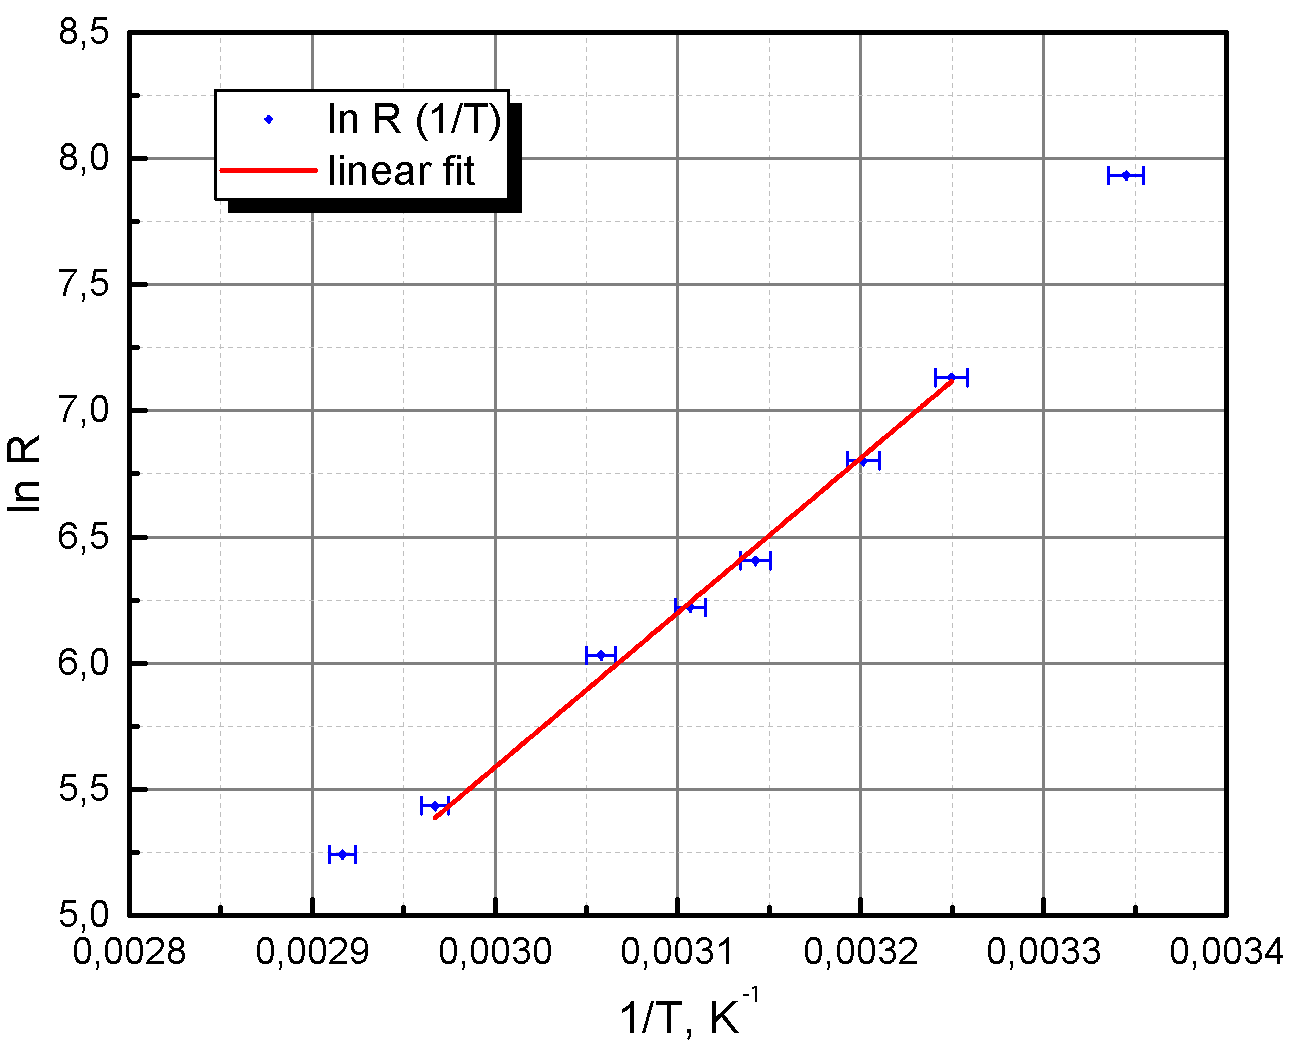
\includegraphics[scale=0.7]{graph.pdf}}    
			\end{floatrow}
		\end{figure}
		Наклон прямой есть $(6200 \pm 200)$ К. Применяя формулу~(\ref{eq:formula}), получаем
		\boxed{$$
			\Delta V = (534 \pm 17)\,\text{мВ}$$}.

\section{Обсуждение результатов и выводы}
	Определили контактную разность потенциалов (p-n)-перехода в полупроводниковом диоде $\Delta V = 534$ мВ с относительной погрешностью в 3\% по результатам измерений температурной зависимости его сопротивления.


\end{document}